\documentclass[12pt]{article}

\usepackage{graphicx} % Required for inserting images

\usepackage[a4paper, top=1cm, left=2cm, right=2cm]{geometry}
\usepackage{setspace}
\usepackage{amsmath,amssymb}
\usepackage{changepage}

\usepackage{enumitem}
\setlist[enumerate]{itemsep=1em}

\usepackage{pgfplots} % plot
\pgfplotsset{compat=1.18}
\usepgfplotslibrary{fillbetween}

\usepackage{booktabs}
\usepackage{tabularx}
\usepackage{float}
\usepackage{array}
\usepackage{caption}
\usepackage{forest}

\usepackage{tikz}
\usetikzlibrary{
    shapes.geometric,
    positioning,
    calc,
    arrows.meta
}

\tikzset{
    entity/.style={
        rectangle,
        draw,
        minimum width=1.8cm,
        minimum height=0.7cm,
        align=center
    },
    weakentity/.style={
        rectangle,
        draw,
        double,
        double distance=2pt,
        minimum width=1.8cm,
        minimum height=0.7cm,
        align=center
    },
    attribute/.style={
        ellipse,
        draw,
        minimum width=1.5cm,
        minimum height=0.65cm,
        align=center
    },
    multivalued/.style={
        ellipse,
        draw,
        double,
        double distance=2pt,
        minimum width=1.5cm,
        minimum height=0.65cm,
        align=center
    },
    derived/.style={
        ellipse,
        draw,
        dashed,
        minimum width=1.5cm,
        minimum height=0.65cm,
        align=center
    },
    relationship/.style={
        diamond,
        draw,
        aspect=2,
        minimum width=1.5cm,
        minimum height=0.8cm,
        align=center
    },
    identifying/.style={
        diamond,
        draw,
        double,
        double distance=2pt,
        aspect=2,
        minimum width=1.5cm,
        minimum height=0.8cm,
        align=center
    },
    % partial key
    partialkey/.style={
        attribute,
        append after command={
            \pgfextra{
                \draw[dashed]
                ([yshift=3pt]\tikzlastnode.south west)
                --
                ([yshift=3pt]\tikzlastnode.south east);
            }
        }
    }
}

\usepackage{listings}
\usepackage{xcolor}

\usepackage{xeCJK}
\setCJKmainfont{Noto Serif CJK TC}
\setCJKmonofont{Noto Sans CJK TC}

\setlength{\parindent}{0pt}
\setlength{\parskip}{0.6em}

\title{Database Management Homework 1}
\author{資管三\quad B13705005宋宇倫\quad B13705011陳芃慈}
\date{}

\begin{document}

\maketitle

\subsection*{2.}

\begin{figure}[h]
\resizebox{1\textwidth}{!}{
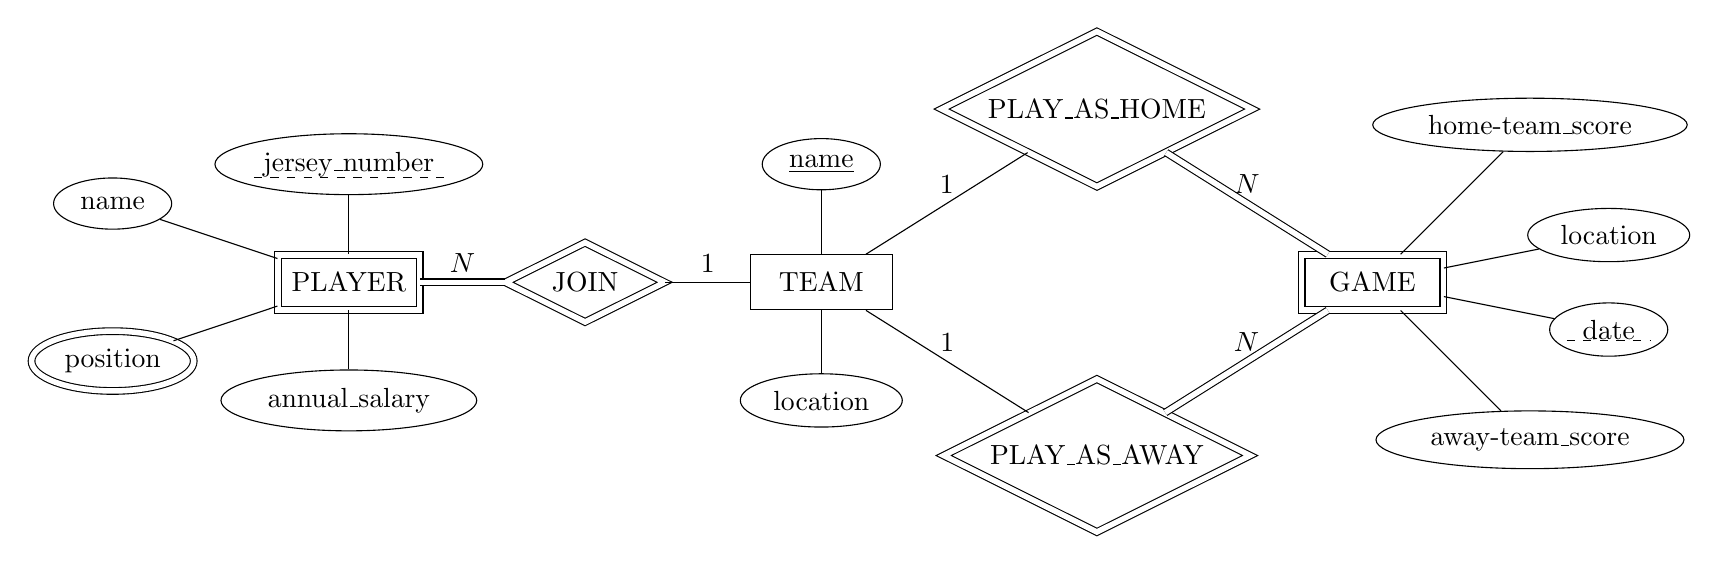
\begin{tikzpicture}
    % team
    \node[entity] (TEAM) at (0, 0) {TEAM};

    \node[attribute] (TEAM_name) at (0,1.5) {\underline{name}};
    
    \node[attribute] (TEAM_loc) at (0,-1.5) {location};

    % player
    \node[weakentity] (PLAYER) at (-6,0) {PLAYER};

    \node[attribute] (PLAYER_name) at (-9, 1) {name};

    \node[partialkey] (PLAYER_jersey) at (-6, 1.5) {jersey\_number};

    \node[multivalued] (PLAYER_pos) at (-9, -1) {position};

    \node[attribute] (PLAYER_salary) at (-6, -1.5) {annual\_salary};

    % game
    \node[weakentity] (GAME) at (7, 0) {GAME};

    \node[attribute] (GAME_loc) at (10, 0.6) {location};
    
    \node[partialkey] (GAME_date) at (10, -0.6) {date};

    \node[attribute] (GAME_home_score) at (9, 2) {home-team\_score};

    \node[attribute] (GAME_away_score) at (9, -2) {away-team\_score};

    % relationship
    \node[identifying] (JOIN) at (-3, 0) {JOIN};

    \node[identifying] (PLAY_AS_HOME) at (3.5, 2.2) {PLAY\_AS\_HOME};

    \node[identifying] (PLAY_AS_AWAY) at (3.5, -2.2) {PLAY\_AS\_AWAY};

    % relationship line
    \draw[double, double distance=2pt]
        (PLAYER) -- node[above] {$N$} (JOIN);

    \draw (JOIN) -- node[above] {$1$} (TEAM);

    \draw (TEAM) -- node[above] {$1$} (PLAY_AS_HOME);

    \draw[double, double distance=2pt]
        (PLAY_AS_HOME) -- node[above] {$N$} (GAME);

    \draw (TEAM) -- node[above] {$1$} (PLAY_AS_AWAY);

    \draw[double, double distance=2pt]
        (PLAY_AS_AWAY) -- node[above] {$N$} (GAME);

    % attr line
    \draw (TEAM) -- (TEAM_name);

    \draw (TEAM) -- (TEAM_loc);

    \draw (PLAYER) -- (PLAYER_name);

    \draw (PLAYER) -- (PLAYER_jersey);

    \draw (PLAYER) -- (PLAYER_pos);

    \draw (PLAYER) -- (PLAYER_salary);

    \draw (GAME) -- (GAME_loc);

    \draw (GAME) -- (GAME_date);

    \draw (GAME) -- (GAME_home_score);

    \draw (GAME) -- (GAME_away_score);

\end{tikzpicture}
}
\caption{Entity-relationship diagram}
\end{figure}

\begin{tikzpicture}[node distance=1.5cm]


\end{tikzpicture}

\medskip

\subsection*{3.}

\begin{figure}[h]
    \centering
    \includegraphics[width=1\textwidth]{hw1-3.png}
    \caption{Relational schema diagram}
    \label{fig:schema}
\end{figure}

\subsection*{4.}

\end{document}
